\subsection{ Discrete and Continuous SpSL Priors}

The spike-and-slab priors \citep{mitchell1988bayesian,george1993variable} are defined as
\begin{align}
    \theta_j | \gamma_j &\sim (1-\gamma_j) \pi_0(\theta_j) + \gamma_j \pi_1(\theta_j) \\
    \gamma_j &\sim \text{Bernoulli}(\eta) \nonumber
\end{align}

When $\pi_0$ is the point-mass at zero, we call the prior a discrete SpSL prior, otherwise we call it a continuous prior. Typically, $\pi_0$ and $\pi_1$ for a continuous SpSL prior can be defined as two Gaussian distributions with a small and a large variance, respectively.

The computation of the posterior inference based on the discrete SpSL prior is often challenging. Several MCMC sampling strategies and stochastic search strategies have been proposed in literature to counter the difficulty. The MCMC sampling of the posterior using the continuous prior can be more efficiently implemented because of the advantage of conjugacy. However, compared to discrete SpSL prior, the continuous prior does not automatically conclude selected coefficients, and extra variable selection steps are required. 

Let the activation function in Equation \eqref{eq:neuronized} be the rectifier linear unit (ReLU) function,
$$ T(t) = \max \{0,t\}.$$
Set $\alpha_0 = 0$, then the activation function $T(\alpha_j - \alpha_0)$ follows an equal mixture of a point mass at zero and the half standard Gaussian. Under this setting, the neuronized prior in Equation \eqref{eq:neuronized} is equivalent to the discrete SpSL distribution with $\eta=\frac{1}{2}$, which is in the form
\begin{align}
    \theta | \gamma & \sim (1-\gamma) \delta_0(\theta) + \gamma \pi(\theta), \\
    \gamma &\sim \text{Bernoulli} (\frac{1}{2}), \nonumber
\end{align}

Figure \ref{fig:SpSL_prior} shows the histogram of $T(\alpha)$, $T(\alpha)w$, and the standard SpSL prior. Here $\tau_w^2 = 1$. As is shown in the figure, the neuronized prior using the ReLU function as activation function is equivalent to the discrete SpSL prior.

\begin{figure}[t]
     \centering
     \begin{subfigure}[b]{0.49\textwidth}
         \centering
         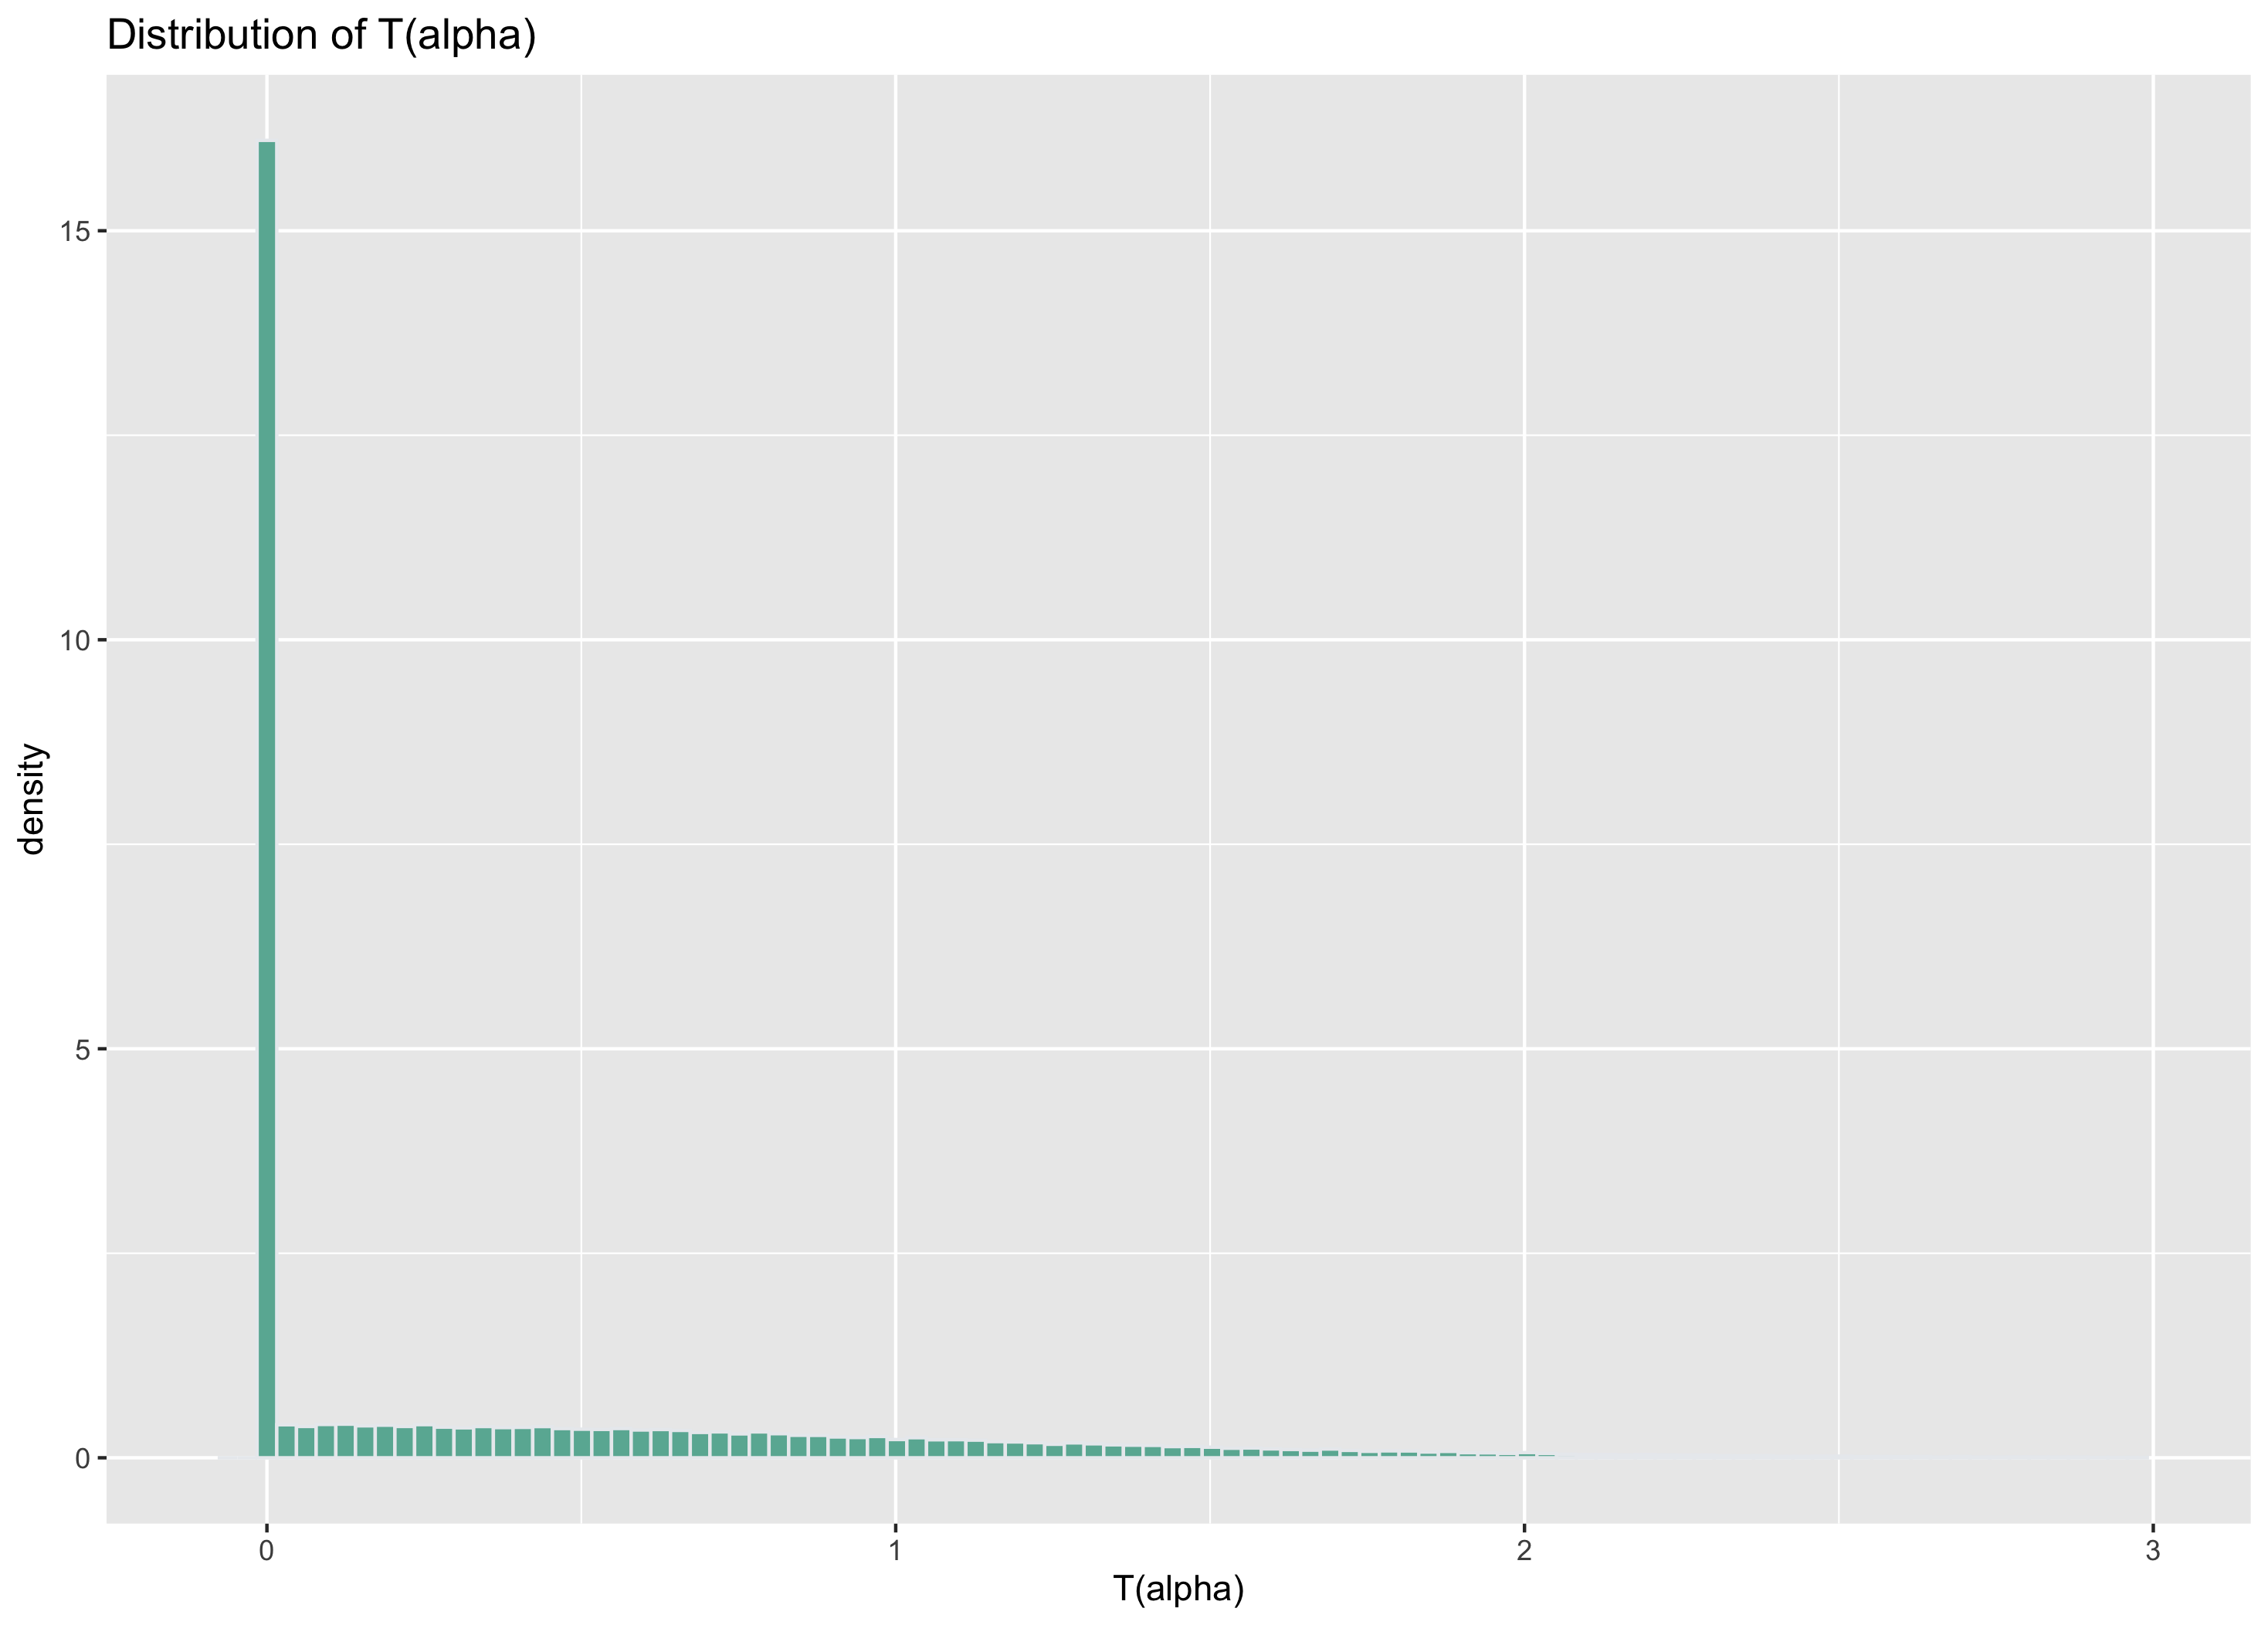
\includegraphics[width=\textwidth]{Figures/SpSLprior1.png}
     \end{subfigure}
     \hfill
     \begin{subfigure}[b]{0.49\textwidth}
         \centering
         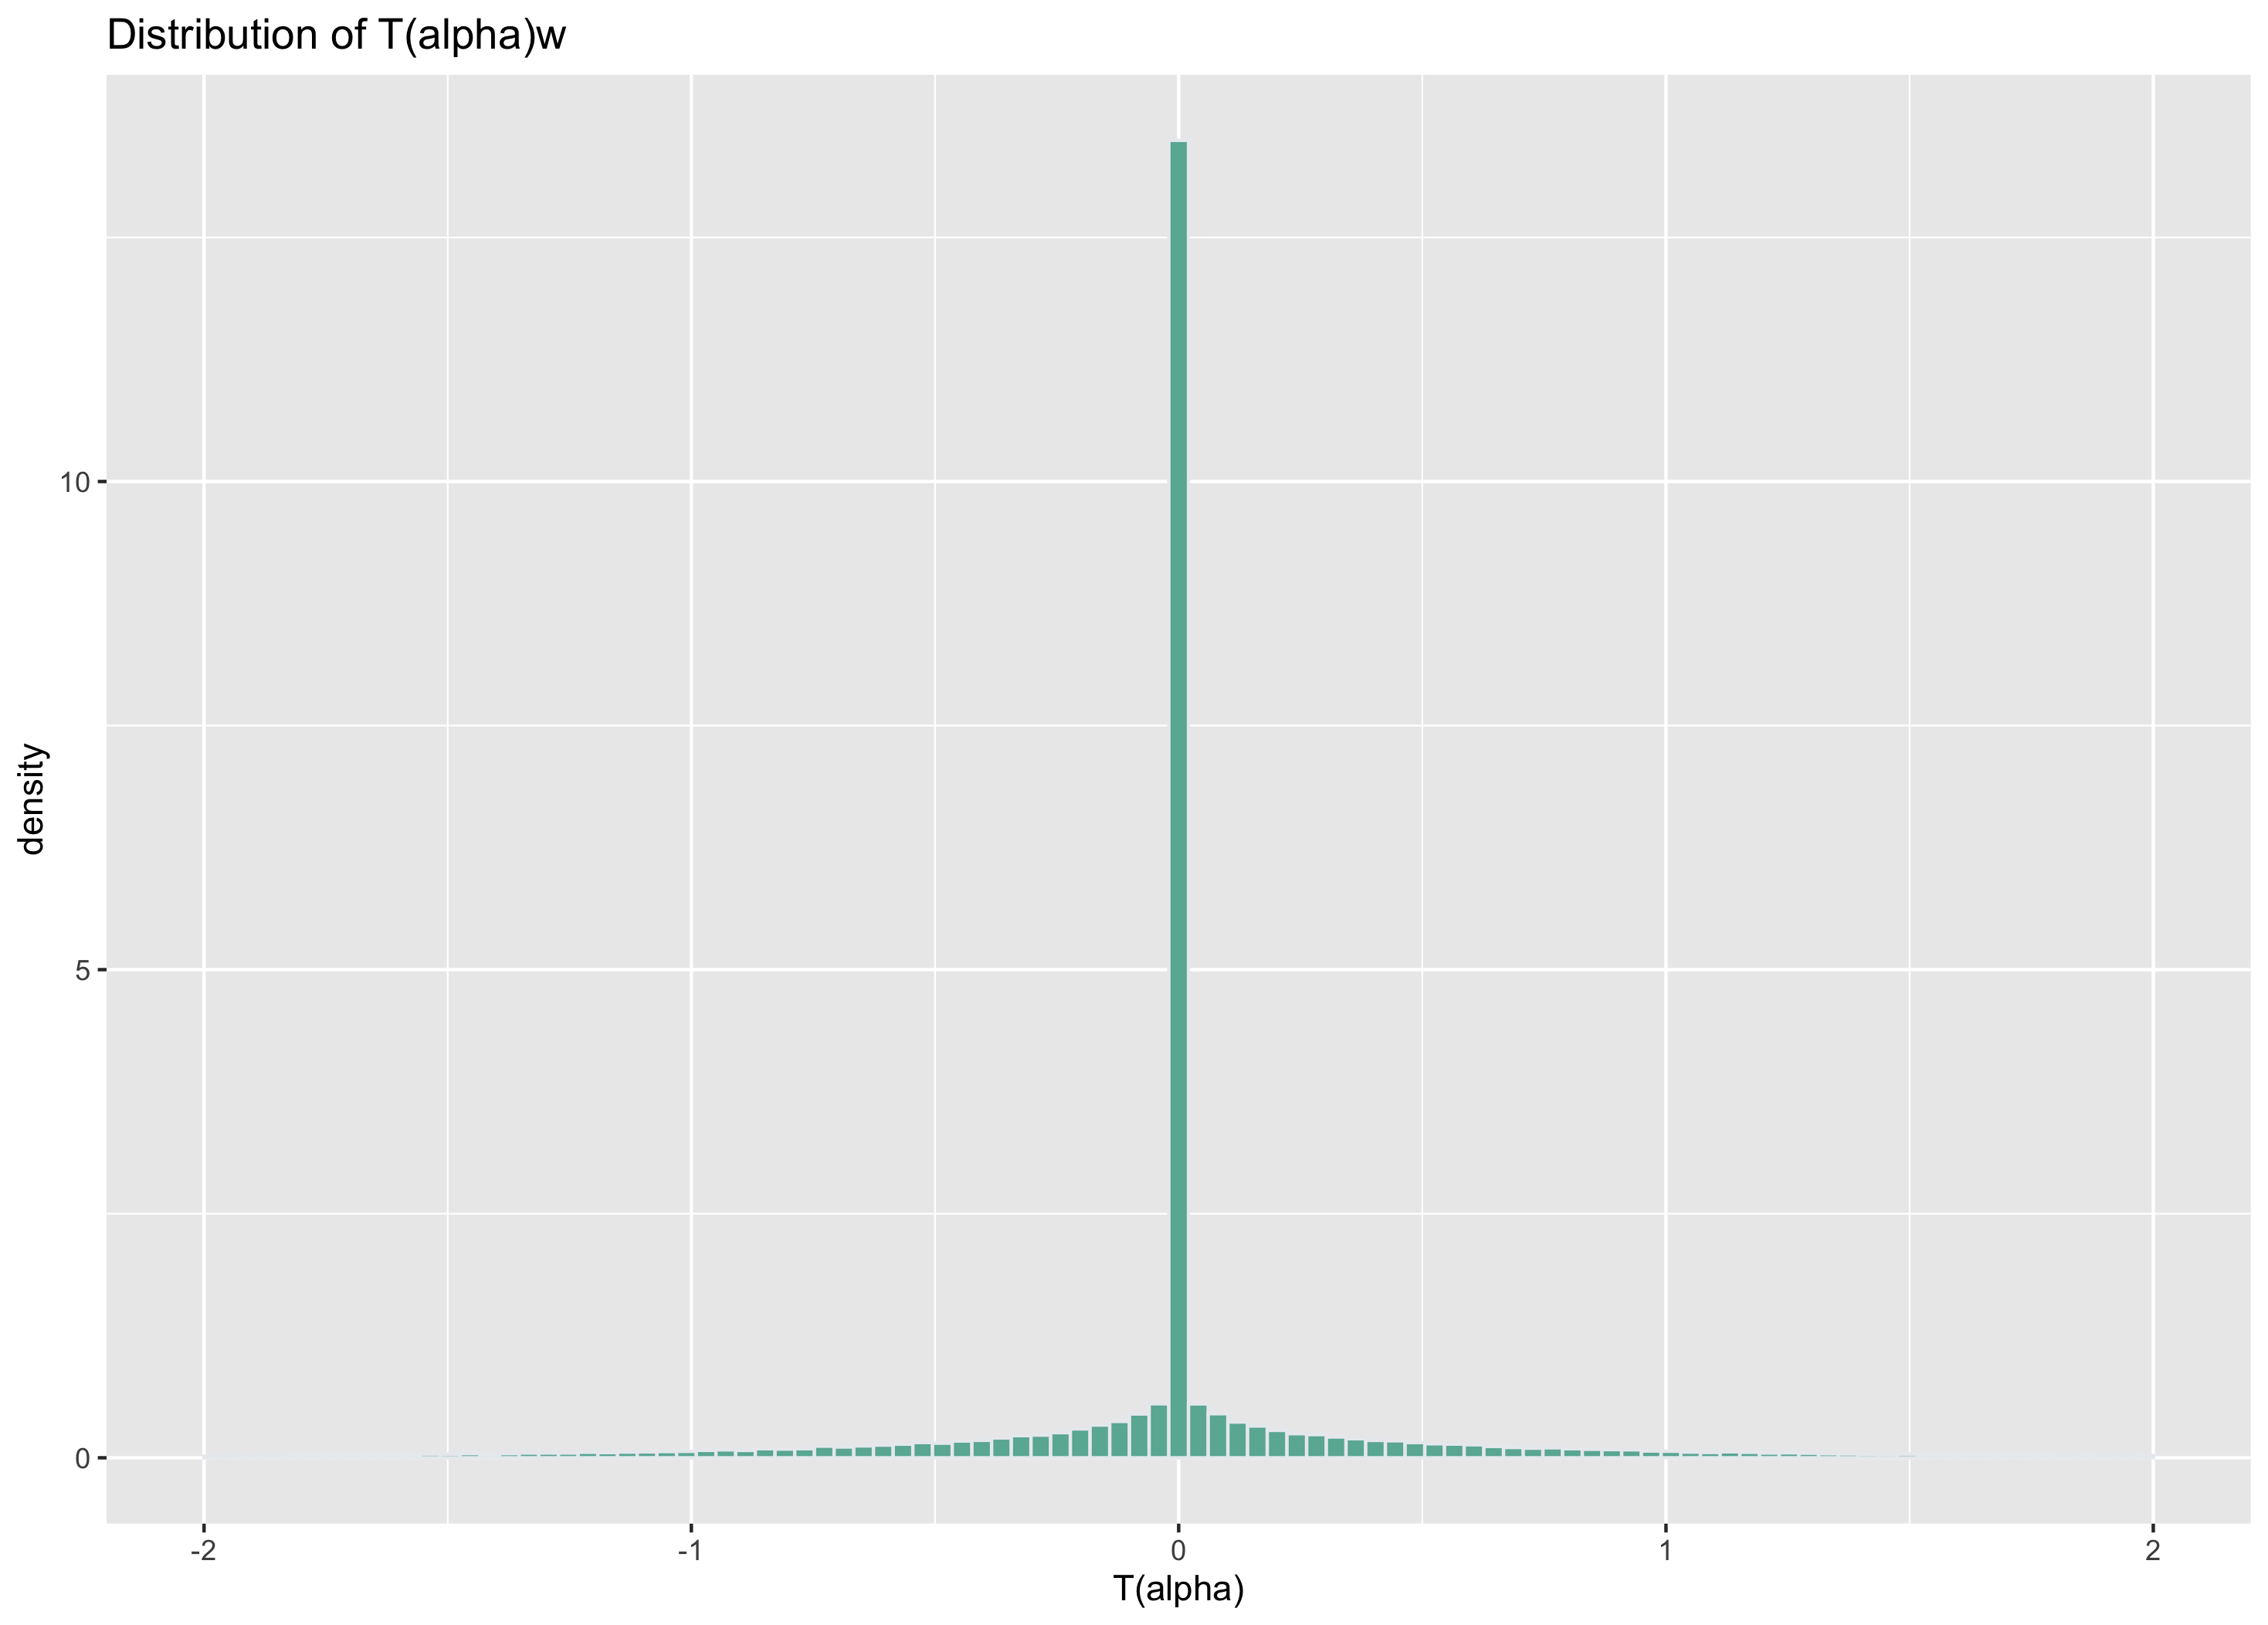
\includegraphics[width=\textwidth]{Figures/SpSLprior2.png}
     \end{subfigure}
     \hfill
     \begin{subfigure}[b]{0.49\textwidth}
         \centering
         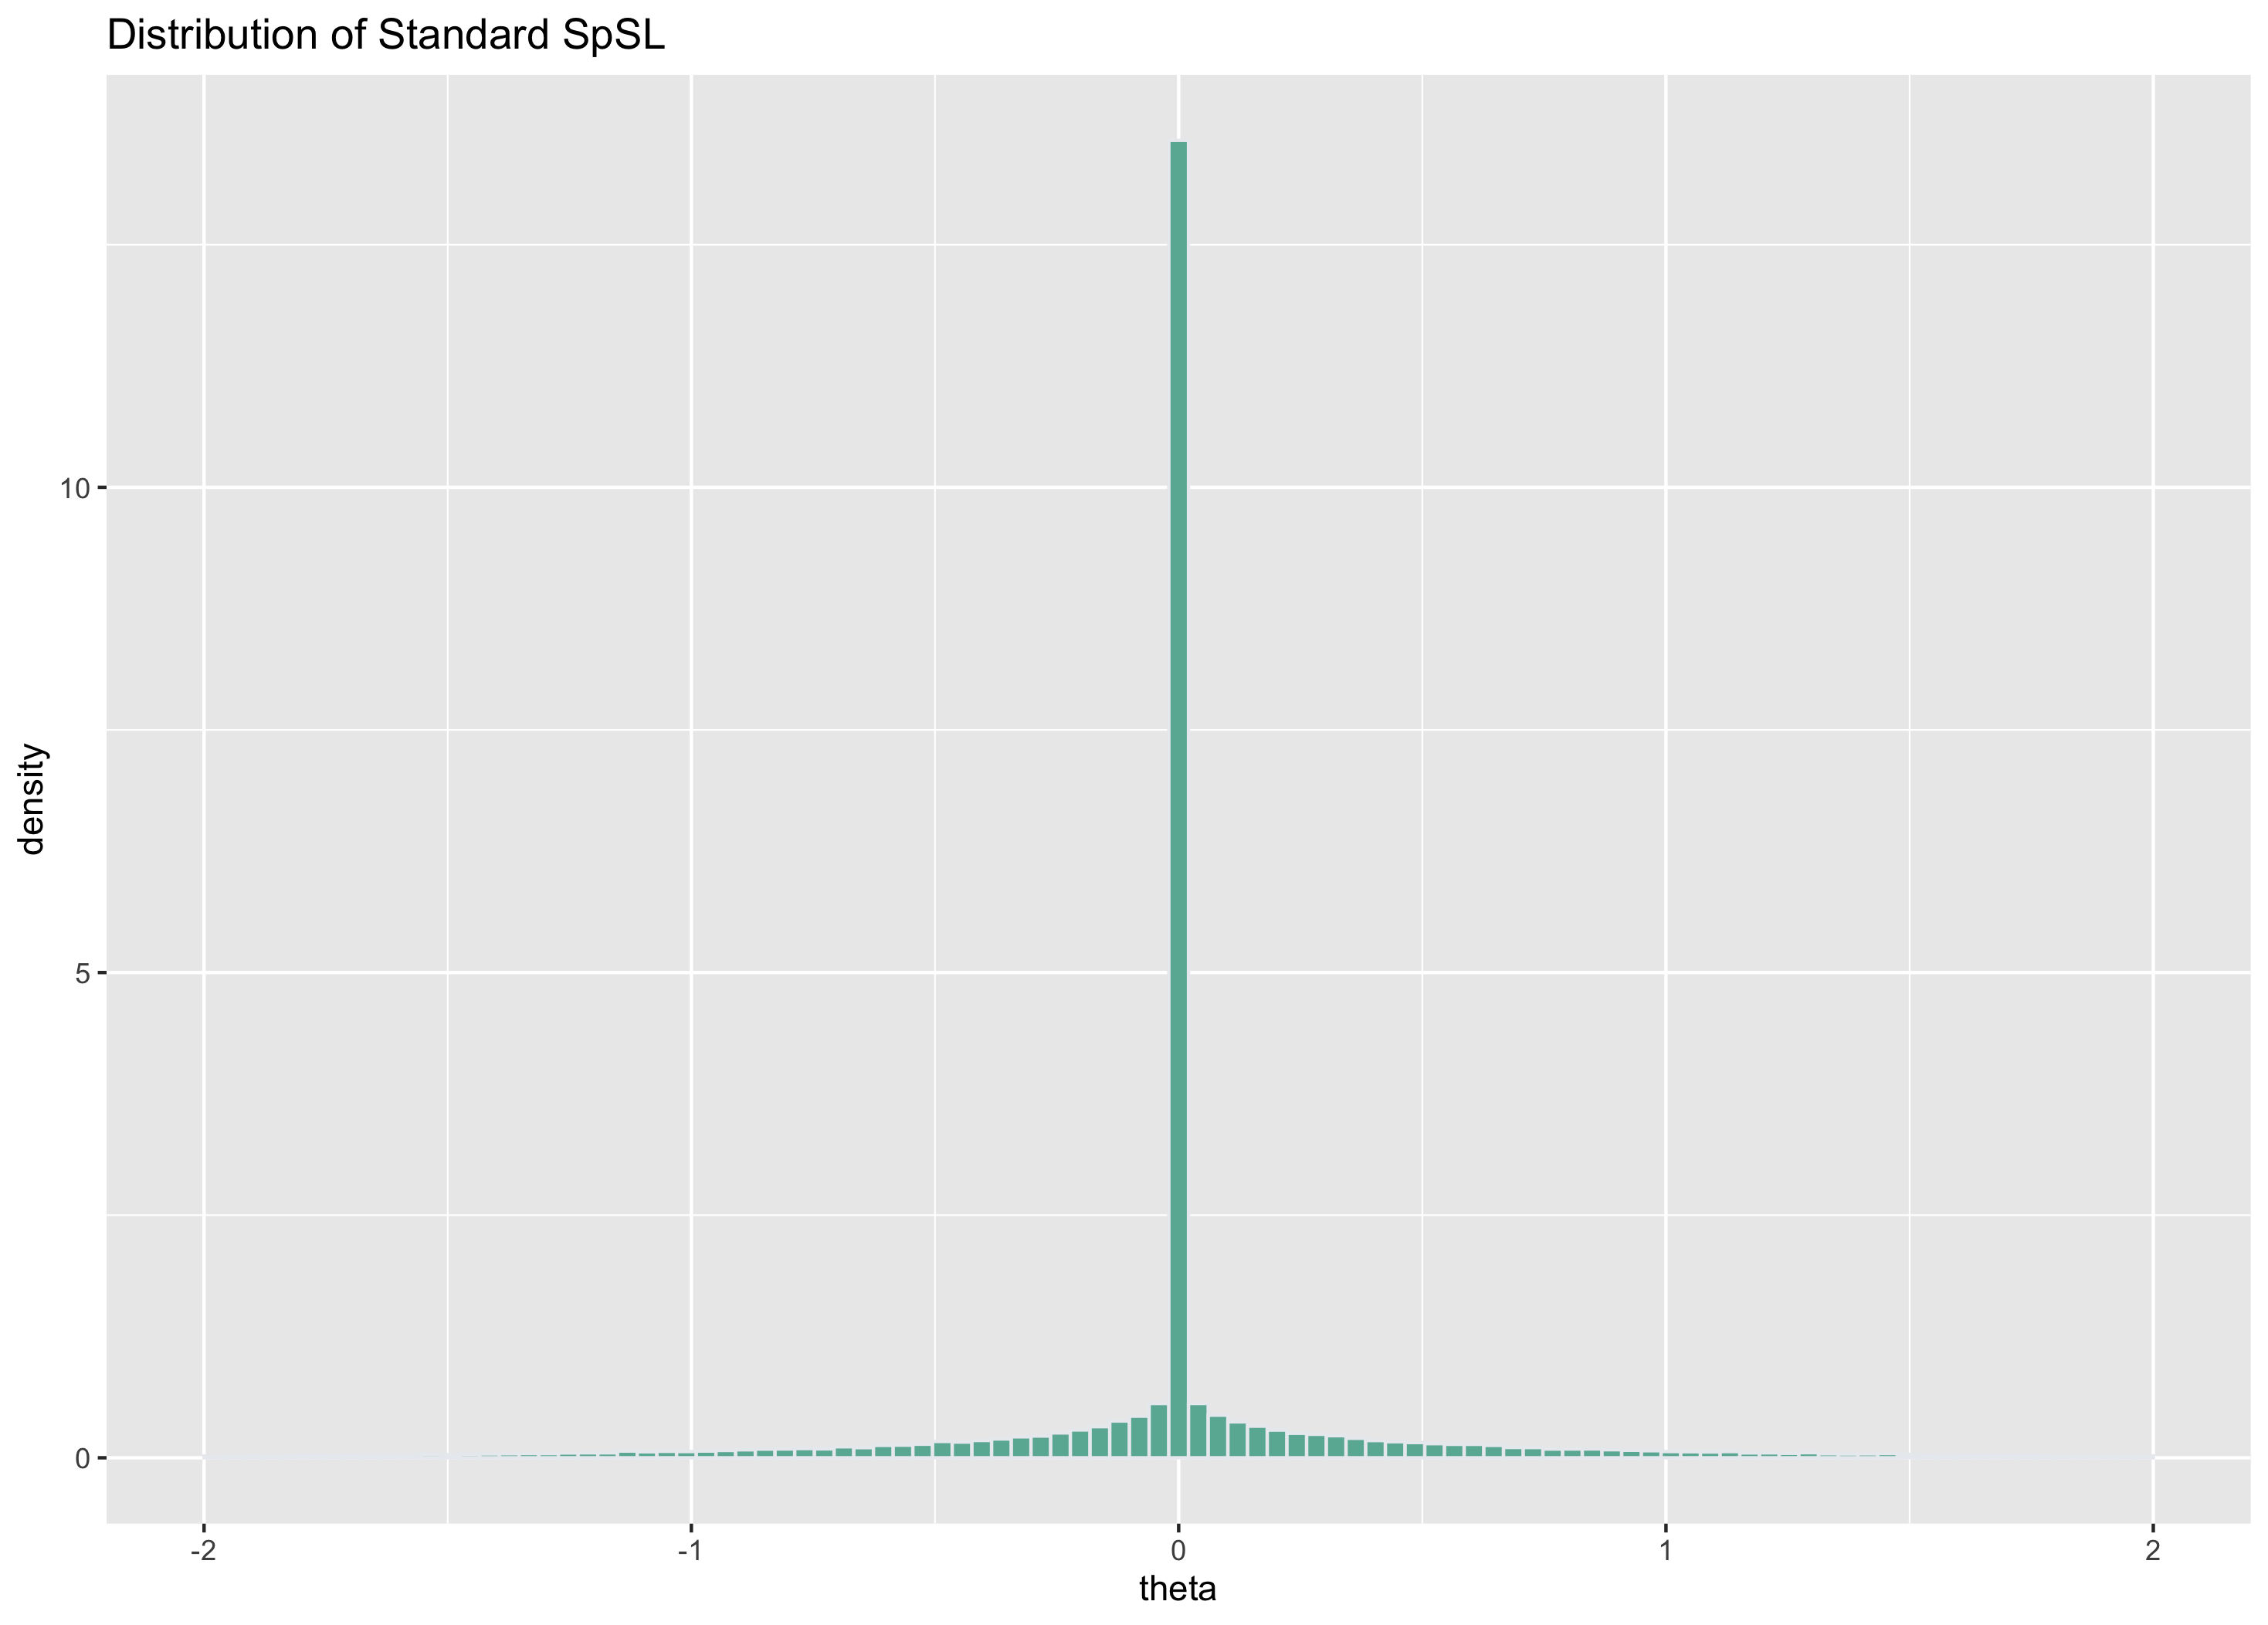
\includegraphics[width=\textwidth]{Figures/SpSLprior3.png}
     \end{subfigure}
        \caption{Histogram of $T(\alpha)$, $T(\alpha)w$, and the standard SpSL prior.}
        \label{fig:SpSL_prior}
\end{figure}

Generally, without the assumption $\alpha_0 = 0$, the neuronized prior with the ReLU activation function gives the same distribution as the standard SpSL prior in Equation \eqref{fig:SpSL_prior} when $\gamma$ is set to be $\gamma \sim \text{Bernoulli}(\Phi(-\alpha_0))$, with $\Phi$ denoting the standard Gaussian CDF. The hyper-parameter $\alpha_0$ controls the probability of sparsity of the prior distribution, 
$$P(T(\alpha_j - \alpha_0) = 0|\alpha_0) = P(\alpha_j < \alpha_0 | \alpha_0) = \Phi(\alpha_0).$$
Conversely, it means that we can choose a desirable level of sparsity with $\alpha_0 = -\Phi^{-1}(\eta)$, for any $\eta \in (0,1)$.

For standard discrete SpSL distribution, as is shown in \citet{scott2010bayes}, a Beta hyper-prior can be put on the sparsity parameter $\eta$,
\begin{equation} \label{eq:spsl_hyper_beta}
    \eta \sim Beta(a_0,b_0),
\end{equation}
where $a_0 = b_0 = 1$ leading to s strong effect on multiplicity correction. If $(a_0,b_0) = (1,p^a)$ for $a>1$, and the number of predictors $p$ increases at a sub-exponential rate of n, $p = O(\exp(n^c))$ for $c<1$, \citet{castillo2012needles} and \citet{castillo2015bayesian} propose that this SpSL procedure achieves model selection consistency and the optimal posterior contraction rate. By adopting a hyper-prior on $\alpha_0$, 
$$ \pi(\alpha_0) \propto \Phi(-\alpha_0)^{a_0-1} (1-\Phi(-\alpha_0))^{b_0 -1} \phi(\alpha_0),$$
the neuronized SpSL prior distribution is identical to the standard SpSL prior in Equation \eqref{fig:SpSL_prior} with the Beta prior \eqref{eq:spsl_hyper_beta} on $\eta$.

Using the ``leaky'' ReLU activation function
$$ T(t) = \max \{ct,t\},$$
where $c$ is a constant $c<1$, we can obtain the continuous SpSL prior from Equation \eqref{eq:neuronized}. 
